%
% $RCSfile: human_body.tex,v $
%
% Copyright (C) 2002-2008. Christian Heller.
%
% Permission is granted to copy, distribute and/or modify this document
% under the terms of the GNU Free Documentation License, Version 1.1 or
% any later version published by the Free Software Foundation; with no
% Invariant Sections, with no Front-Cover Texts and with no Back-Cover
% Texts. A copy of the license is included in the section entitled
% "GNU Free Documentation License".
%
% http://www.cybop.net
% - Cybernetics Oriented Programming -
%
% http://www.resmedicinae.org
% - Information in Medicine -
%
% Version: $Revision: 1.1 $ $Date: 2008-08-19 20:41:07 $ $Author: christian $
% Authors: Christian Heller <christian.heller@tuxtax.de>
%

\subsubsection{Human Body}
\label{human_body_heading}
\index{Human Body}
\index{Sensoric Organs}
\index{Motoric Organs}
\index{Human Senses}
\index{Nerve Cell}
\index{Muscle Cell}
\index{Information Reception}
\index{Information Sending}

Figure \ref{human_figure} shows parts of the animalic nerve system of a human
being. \emph{Sensoric} organs are used for information input; \emph{motoric}
organs for information output.

\begin{figure}[ht]
    \begin{center}
        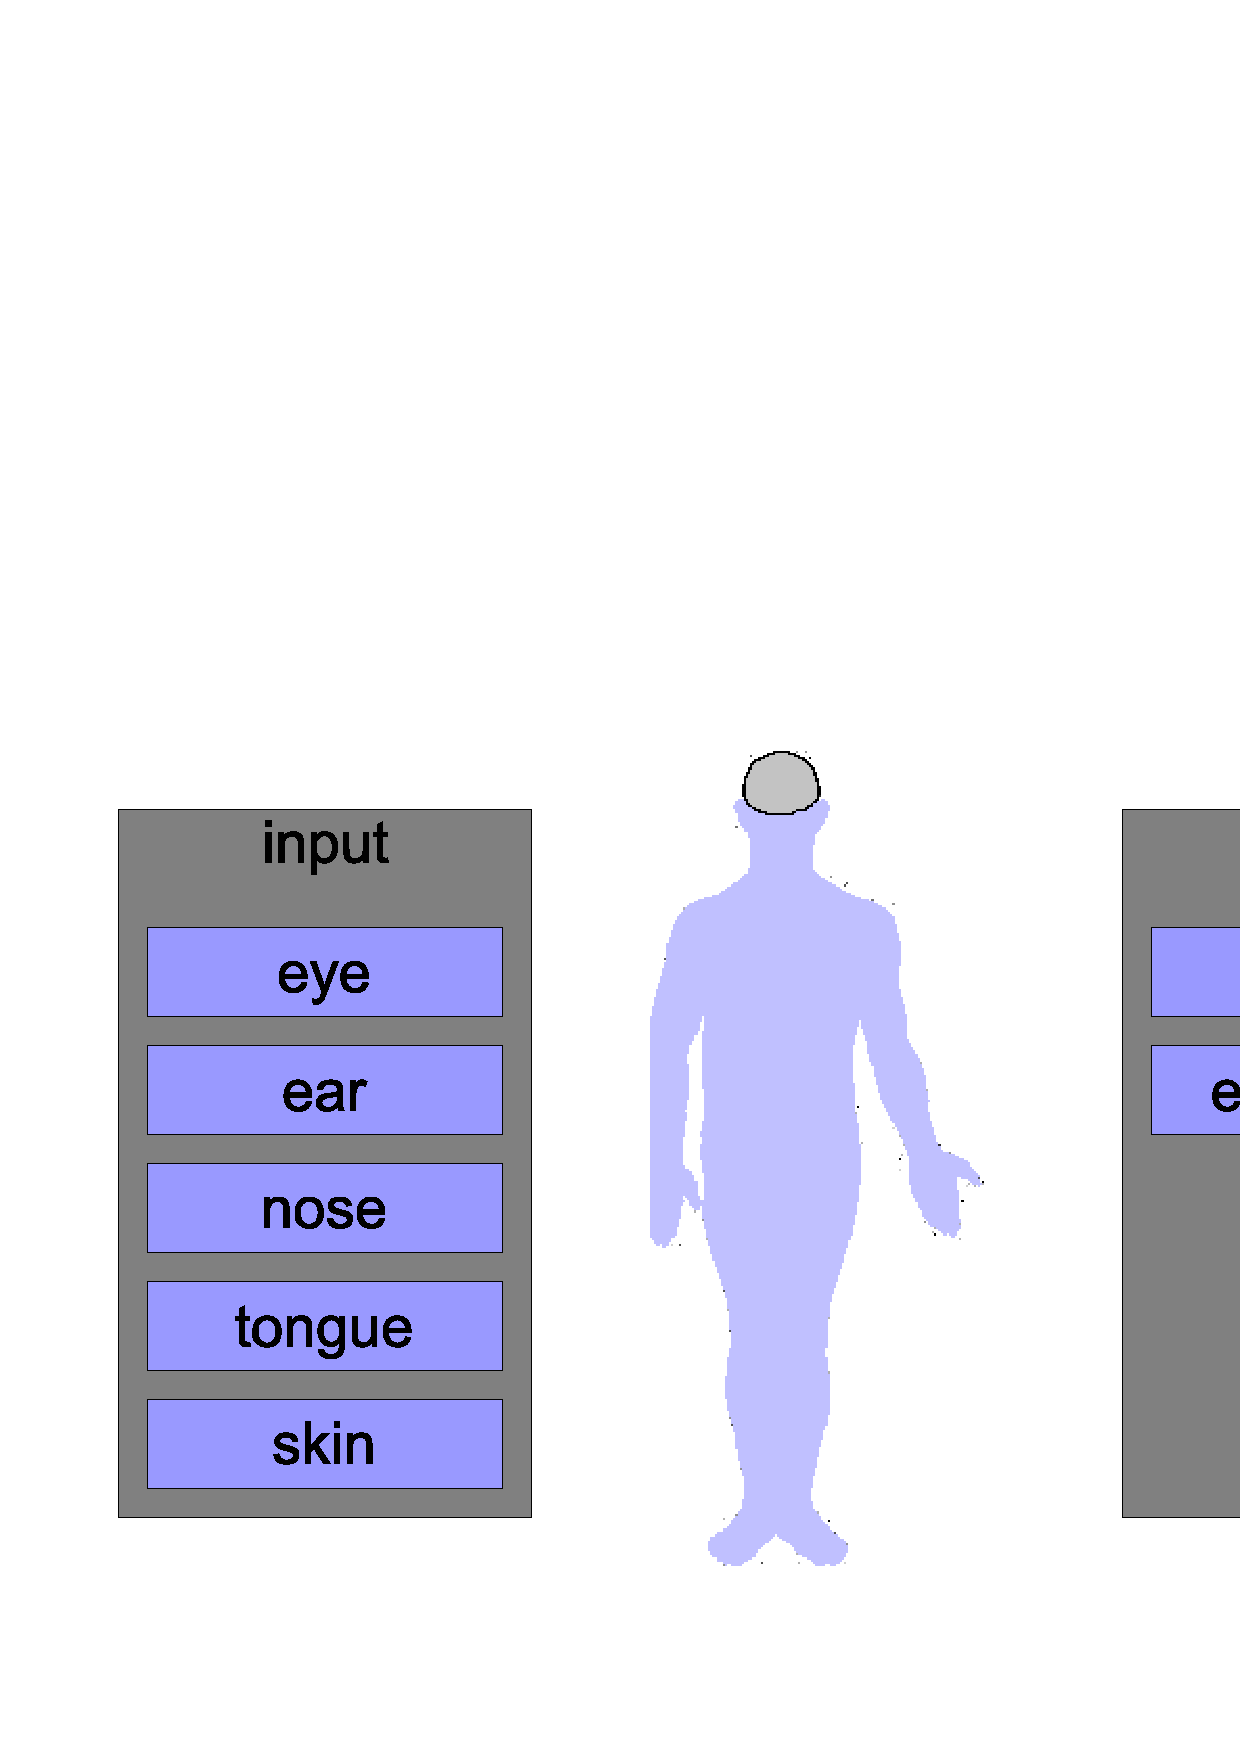
\includegraphics[scale=0.3,angle=-90]{graphic/human.pdf}
        \caption{Human Body with Sensoric and Motoric Organs}
        \label{human_figure}
    \end{center}
\end{figure}

The five (seven) human senses were already shown in table \ref{senses_table}.
They are able to receive signals which are transported by different mediums.
The transport mechanisms rely on various physical and chemical \emph{Effects},
as shown in table \ref{effects_table}. Each sense is represented by an
\emph{Organ}. The optic cells of the retina of an \emph{Eye} bundle light
stimuli which the optic nerve forwards as electrical signal to the brain. The
inner \emph{Ear} transforms oscillation frequencies of sound-waves into
electrical signals to send on to the brain. And so forth.

\begin{table}[ht]
    \begin{center}
        \begin{footnotesize}
        \begin{tabular}{| p{30mm} | p{50mm} | p{25mm} |}
            \hline
            \textbf{Effect} & \textbf{Science} & \textbf{Sense}\\
            \hline
            Oscillation, Wave & Physics, Mechanics & Seeing, Hearing\\
            \hline
            Density, Temperature & Physics, Mechanics, Thermodynamics & Tactile\\
            \hline
            Aroma & Chemistry & Smelling, Tasting\\
            \hline
        \end{tabular}
        \end{footnotesize}
        \caption{Effects as Basis of Sensing}
        \label{effects_table}
    \end{center}
\end{table}

While the \emph{Reception} of information is based on \emph{Nerve Cells}, it is
\emph{Muscle Cells} which are responsible for information \emph{Sending}.
Humans communicate for example through visual \emph{Gestures} using their
\emph{Extremities} or through acoustical \emph{Talking} using their
\emph{Larynx}/ \emph{Vocal Chords}. The latter, too, is based on muscle
activity.
